\chapter{Cross-Plattform-Entwicklung mit Xamarin}
  Xamarin ist 2011 infolge der Entlassung des fr�heren Teams zur Entwicklung von Mono durch Novell entstanden.
Es ist ein unabh�ngiges Unternehmen, aber arbeitet eng mit Microsofts .NET-Team zusammen. Es
gibt eine Partnerschaft zwischen Microsoft und Xamarin, die dazu f�hrt, dass Visual-Studio-Entwickler 
durch Xamarins Produkte zur Entwicklung von Apps f�r iOS und Android unterst�tzt werden. Im Zuge der 
 Partnerschaft k�nnen MSDN-Abonnenten au�erdem kostenlos auf den Kurs Xamarin University zugreifen, 
 der dabei helfen soll, innerhalb kurzer Zeit zum Experten der Xamarin-Tools zu werden \cite{MX}.
\\Das Entwickeln in einer einheitlichen Programmiersprache ist nicht der einzige Vorteil von
Xamarin.
 Xamarin.Forms ist ein m�chtiges Feature, mit dem man nicht nur die Anwendung in C\# entwickeln
 kann, sondern man auch den gr��ten Teil des Codes gemeinsam f�r alle drei Zielplattformen nutzen
 kann. Man kann mit Xamarin.Forms in einem Projekt gleichzeitig f�r iOS, Android und Windows Phone
 entwickeln und alle drei Produkte haben am Ende bis zu 70\% gemeinsamen Code und nur 30\%
 plattformspezifischen Code.

\section{Getting Started mit Xamarin}
Um Xamarin benutzen zu k�nnen, braucht man einen kostenpflichtigen Account. Es gibt verschiedene
Arten von Accounts, die mit unterschiedlichen Features verbunden sind.
\begin{itemize} 
  \item Indie Account (\$25 im Monat)\\Studenten k�nnen es kostenlos
  beantragen. Im Paket ist die Entwicklungsumgebung von Xamarin, das Xamarin Studio, enthalten.
  Xamarin.iOS und Xamarin.Android kommen ebenso mit dem Indie Account mit, sowie das
  plattform�bergreifende Werkzeug, Xamarin.Forms. Man kann mit diesem Account noch
  Anwendungen in die verschiedenen App-M�rkte deployen.
  \item Business Account (\$83 im Monat)\\Wer professionell Xamarin Apps entwickeln m�chte, kommt an
  den Business Account nicht herum. In diesem Benutzerkonto sind alle Features von Indie enthalten
  plus zus�tzliche Business Features und das wichtigste, Visual Studio Einbindung und privates Email Support von Xamarin Experten.
  \item Enterprise Account (\$158)\\Im Enterprise Account sind viele weitere Features enthalten, wie
  z.B. die Anbindung einer verschl�sselten lokalen Datenbank.
\end{itemize}
Bevor man mit der App Entwicklung mit Xamarin anfangen kann, m�ssen einige Voraussetzungen erf�llt
werden.\\Wenn man f�r iOS oder Mac OS X entwickeln m�chte, wird ein Mac Rechner vorausgesetzt.
Auf einem Mac kann man mit Xamarin Studio, mittels Xamarin.iOS und Xamarin.Android,
plattform�bergreifend f�r iOS und Android entwickeln. Es reichen ein Mac Rechner und ein Xamarin
Indie Account.
\\Auf einem Windows PC kann man nur f�r Android und Windows Phone entwickeln. Eventuell
kann man einen Mac Rechner als Build Server (Macintosh Build Host mit Apples SDK) benutzen, um unter
Windows Apps f�r iOS entwickeln zu k�nnen (siehe Abb.\ref{fig:abb16}).
Daf�r ist allerdings mindestens Business Account erforderlich.
\\Um f�r die drei meist verbreiteten mobilen Betriebssystemen
(Android, iOS und Windows Phone) plattform�bergreifend entwickeln zu k�nnen, werden zwei Rechner
(ein Mac und ein Windows PC) und den Xamarin Business Account ben�tigt. Mit dem Business Account
l�sst sich Xamarin als Plugin in Visual Studio einbinden.
\begin{figure}[!h]
\centering
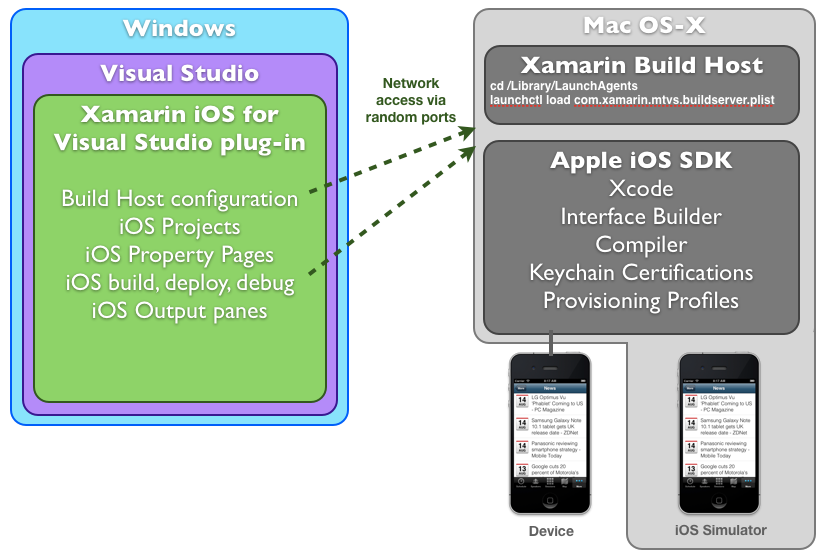
\includegraphics[scale = 0.3]{graphics/Macintosh_Build_Host.png}
\caption{Xamarin unter Windows mit einem Macintosh Build Server (Quelle:\cite{XiOS})}
\label{fig:abb16}
\end{figure}

Im Folgenden werden die drei wichtigsten Bibliotheken von Xamarin vorgestellt. 
Mit Xamarin.iOS/Xamarin.Android erstellte Programme stehen nativen Anwendungen in nichts nach und
k�nnen problemlos in App- bzw. Play- Store eingestellt werden. Da es sich sehr der nativen
App-Programmierung �hnelt, ist der Einstieg in Xamarin.iOs und Xamarin.Android reibungslos f�r
erfahrene Entwickler. Im Gegensatz zu der �blichen App Entwicklung, bei der
unterschiedliche Programmiersprachen (Objective-C und Java) verwendet werden, wird bei Xamarin.iOS
und Xamarin.Android ausschlie�lich C\# benutzt.
\\Die plattform�bergreifende App-Entwicklung mit Xamarin geht noch weiter. Mit Xamarin.Forms lassen 
sich Apps f�r iOS, Android und Windows Phone mit gemeinsamen Code erstellen. Xamarin.Forms ist jedoch 
nicht f�r alle Typen von Anwendungen geeignet.
\section{Xamarin.iOS}
Mit Xamarin.iOS bietet Xamarin die M�glichkeit, native Apps f�r iOS zu entwickeln. Um Xamarin.iOS benutzen zu k�nnen,
ben�tigt man:
\begin{itemize}
  \item das aktuelle iOS SDK
  \item die letzte Version von Xcode
  \item Mac OS X 10.9.3+
\end{itemize}
Unter Mac OS werden Xamarin Apps mit der Entwicklungsumgebung Xamarin Studio entwickelt. Bevor man
eine iOS App auf einem mobilen Endger�t deployen und testen kann, muss man einen Apple Developer
Account haben. Dieser Account ist auch erforderlich, wenn man Apps in den App
Store stellen m�chte.
Der Ahead-Of-Time (AOT) Compiler kompiliert Xamarin.iOS Apps direkt zu nativen ARM Assemblercode, mit anderen Worten, kann man mit Xamarin native iOS Apps erstellen. Mit Xamarin.iOS hat man die iOS SDK von Apple in C\# mit .NET Namenskonventionen. Xamarin bietet somit Zugriff auf alle iOS APIs. Dank eines automatischen Binding-Generators k�nnen existierender Objective-C Code, sowie Frameworks und
benutzerdefinierte Controls problemlos in einer Xamarin App benutzt werden. Wenn man iOS Apps
mittels Visual Studio entwickelt, muss man die App auf dem Macintosh Build Host simulieren, da es
auf Windows keinen iOS Simulator gibt.

\cite{XiOS}
